\begin{figure}[htb]
    \centering
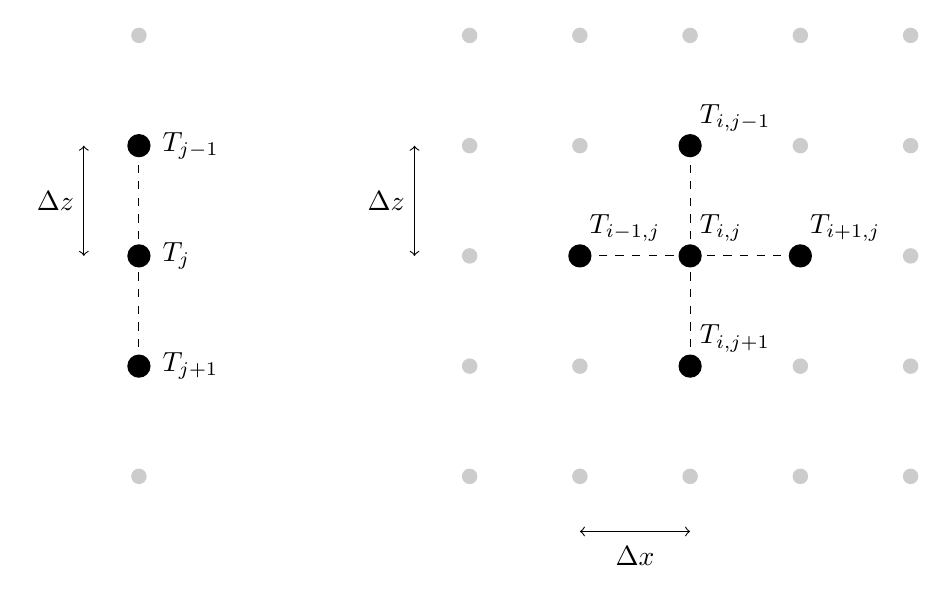
\begin{tikzpicture}[scale=1.4]
    \begin{scope}
        % Background grid nodes (faded)
        \foreach \k in {-2,2} {
            \fill[gray!40] (0,-\k) circle (2pt);
        }

        % Stencil nodes
        \fill (0,0) circle (3pt) node[right,xshift=5] {$T_{j}$};
        \fill (0,1) circle (3pt) node[right,xshift=5] {$T_{j-1}$};
        \fill (0,-1) circle (3pt) node[right,xshift=5] {$T_{j+1}$};

        % Dashed connections
        \draw[dashed] (0,0) -- (0,1);
        \draw[dashed] (0,0) -- (0,-1);

        % Delta z annotation
        \draw[<->] (-0.5,0) -- (-0.5,1) node[midway,left] {$\Delta z$};
    \end{scope}

    \begin{scope}[xshift=5cm]
        % Background grid (faded)
        \foreach \x in {-2,-1,0,1,2} {
            \foreach \z in {-2,-1,0,1,2} {
                \fill[gray!40] (\x,\z) circle (2pt);
            }
        }

        % Stencil nodes
        \fill (0,0) circle (3pt) node[right,yshift=10] {$T_{i,j}$};
        \fill (1,0) circle (3pt) node[right,yshift=10] {$T_{i+1,j}$};
        \fill (-1,0) circle (3pt) node[right,yshift=10] {$T_{i-1,j}$};
        \fill (0,1) circle (3pt) node[right,yshift=10] {$T_{i,j-1}$};
        \fill (0,-1) circle (3pt) node[right,yshift=10] {$T_{i,j+1}$};

        % Dashed stencil connections
        \draw[dashed] (0,0) -- (1,0);
        \draw[dashed] (0,0) -- (-1,0);
        \draw[dashed] (0,0) -- (0,1);
        \draw[dashed] (0,0) -- (0,-1);

        % Delta z annotation
        \draw[<->] (-2.5,0) -- (-2.5,1) node[midway,left] {$\Delta z$};
        \draw[<->] (-1,-2.5) -- (0,-2.5) node[midway,below,yshift=-2pt] {$\Delta x$};
    \end{scope}
\end{tikzpicture}
\caption{Stencils are the constructed connections between nodes used in finite difference approximations.  (a) One-dimensional finite difference stencil for the first and second derivative.  (b) Five-point stencil for the two-dimensional, first-derivative (gradient and divergence) or second-derivative (Laplacian).}
\label{fig:fdstencils}
\end{figure}